%! TEX root = main.tex

In this subsection, we conducted spectral analysis on the cylinder flow to extract frequencies embedded in the simulation results.
Fluid flow is a dynamical system, and how information (or signals) propagates in time plays an important role.
Information with different frequencies advances at different speeds in the temporal direction, and the superposition of information forms complicated flow patterns over time.
Spectral analysis reveals frequencies and corresponding information---which is called {\it dynamic modes} in fluid dynamics.
By comparing the spectral results against PetIBM, we examined how well/badly the data-driven PINN learned information with different frequencies.

We used Koopman analysis \cite{chen_variants_2012,rowley_spectral_2009} to generate the spectral results.
When having time-series solutions of a dynamical system but not knowing the exact propagation mechanism in the temporal direction, Koopman analysis helps identify the system's characteristics, including frequencies and complex-valued dynamic modes.
Here we skip the details of the Koopman analysis.
Please refer to {\it the method of snapshots} in reference \cite{chen_variants_2012} for the theory and the algorithms we used.

Given $m+1$ flow snapshots with a uniform time spacing $\Delta t$: $\vec{g}_0$, $\vec{g}_1$, $\dots$, $\vec{g}_m \in \mathbb{R}^{N}$, our goal is to express these solutions as the superpositions of $m$ dynamic modes:
\begin{equation}\label{eq:discrete-dmd}
    \vec{g}_k
    =
    \sum\limits_{j=1}^{m}
    \vec{v}_j
    \exp\left(\left( \alpha_j + 2 \pi f_j i\right) k \Delta t\right)
    ,\quad
    k = 0, 1, \cdots, m
\end{equation}
which is a discretized version of the following continuous complex-valued series expansion:
\begin{equation}\label{eq:continuous-dmd}
    \vec{g}(\vec{x}, t)
    =
    \sum\limits_{j=1}^{m}
    \vec{v}_j(\vec{x})
    \exp\left(\left( \alpha_j + 2\pi f_j i\right) t\right)
\end{equation}
$\vec{v}_j \in \mathbb{C}^{N}$ denotes the $j$-th dynamic mode.
$\alpha_j \in \mathbb{R}$ is called the growth rate because $\exp\left(\alpha_j t\right)$ controls the damping/growth of the $j$-th mode over time.
$f_j \in \mathbb{R}$ is the frequency associated with the $j$-th mode. 
$i$ is the imaginary unit.
Note that for a periodic flow pattern (such as vortex shedding), the growth rate $\alpha_j$ must be zero because no mode can become stronger or weaker.

After applying the Koopman analysis, the outcome provides the following series expansion of the solutions:
\begin{equation}\label{eq:koopman}
    \vec{g}_k
    =
    \sum\limits_{j=1}^{m}
    \lambda_j^k \vec{v}_j
    ,\quad
    k = 0, 1, \cdots, m
\end{equation}
where $\lambda_j \in \mathbb{C}$ is called $j$-th Koopman eigenvalue, and $\lambda_j^k$ is $\lambda_j$ to the power of $k$.
$\vec{v}_j$ is the $j$-th Koopman eigenvector and is the same as the $j$-th dynamic mode in equation \eqref{eq:discrete-dmd}.
Equating equation \eqref{eq:discrete-dmd} and \eqref{eq:koopman} allows us to calculate the growth rates and frequencies using the Koopman eigenvalues:
\begin{equation}
    \left\{
        \begin{array}{l}
            \alpha_j = \frac{1}{\Delta t} \mathfrak{Re}\left(\ln\left(\lambda_j\right)\right) \\
            f_j = \frac{1}{2\pi\Delta t} \mathfrak{Im}\left(\ln\left(\lambda_j\right)\right) \\
        \end{array}
    \right.
\end{equation} 

We analyzed the results from PetIBM and the data-driven PINN in $t\in$$[125$, $140]$, which contains about three full cycles of vortex shedding.
A total of $76$ solution snapshots were used from each solver.
The time spacing is $\Delta t = 0.2$.
The Koopman analysis would result in $75$ modes.
Since the snapshots cover three full cycles, we would expect only $25$ distinct frequencies and $25$ nontrivial modes---only $25$ out of $76$ snapshots are distinct.
However, this expectation only happens when the data are free from noise and numerical errors and when the number of three periods is exact.
We would see more than $25$ distinct frequencies and modes if the data were not ideal.
In $t \in [125, 140]$, the data-driven PINN was trained against PetIBM's data, so we expected to see similar spectral results between the two solvers.

Figure \ref{fig:koopman-eigval-dist} shows the distributions of the Koopman eigenvalues, $\lambda_j$, on the complex plane.
The color of each dot represents the normalized strength of the corresponding mode, defined as:
\begin{equation}
    \text{normalized strength of the }j\text{-th mode}
    \equiv
    \frac{\lVert \vec{v}_j \rVert \sqrt{m+1}}{\sqrt{\sum\limits_{k=0}^{m}\lVert\vec{g}_k\rVert^2}}
\end{equation}
The star marker denotes the mode with $f_j=0$: a steady or time-independent mode.
This mode usually has much higher strength than others, so we excluded it from the color map and annotated its strength on each figure.
Koopman eigenvalues come as complex conjugate pairs, so the modes are symmetric with respect to the real-number axis. 
A conjugate pair has an opposite sign in $f_j$ but has the same physical frequency (e.g., $\exp(2\pi f_jt)$ and $\exp(2\pi (-f_j)t)$ both propagate at the same frequency physically).

We also plotted a circle with a radius of one on each figure.
As flow has already reached a fully periodic regime, the growth rates $\alpha_j$ should be zero, that is, $\mathfrak{Re}\left(\ln\left(\lambda_j\right)\right) = \ln\left(\lvert \lambda_j \rvert\right) = 0$.
In other words, $\lvert \lambda_j \rvert = 1$, meaning all $\lambda_j$ were expected to fall on this circle on the complex plane.
If a mode falls inside the circle, it has a negative growth rate, and its contribution to the solution diminishes over time.
Similarly, a mode falling outside the circle has positive growth over time.

\begin{figure}[hbt!]
    \centering
    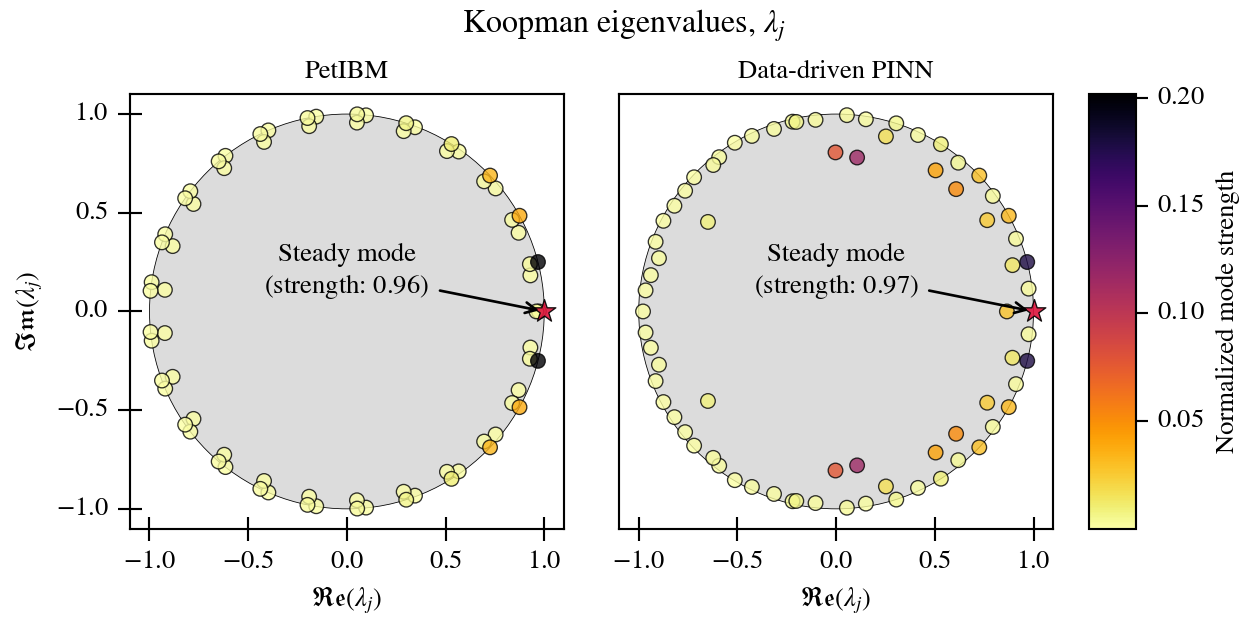
\includegraphics[width=0.975\linewidth]{cylinder-2d-re200/koopman/koopman_eigenvalues_complex}
    \caption{2D Cylinder, $Re=200$: Koopman eigenvalue distribution on the complex plane}
    \label{fig:koopman-eigval-dist}
\end{figure}

On the complex plane, all $\lambda_j$ of PetIBM fall onto the circle or close to the circle (on the left in figure \ref{fig:koopman-eigval-dist}).
Though PetIBM's plot shows $75$---rather than $25$---distinct $\lambda_j$ and modes, modes are evenly clustered into 25 groups.
Each group has three modes, among which one or two modes fall on the circle, while the remaining one(s) falls inside but very close to the circle.
Modes within each group have a similar $\lambda_j$, and the one precisely on the circle has significantly higher strength than other modes (if not all modes in the group are weak).
Due to the numerical errors in PetIBM's solutions, data in a vortex period are similar to but not exactly the same as those in another period.
The strong modes falling precisely on the circle may represent the period-averaged flow patterns and are the $25$ modes we expected in the previous paragraphs. 
The effect of numerical errors was filtered out from these modes.
We call these 25 modes primary modes and all other modes secondary modes.
Secondary modes are mostly weak and may come from the numerical errors in the PetIBM simulation.
The plot shows these secondary modes are slightly dispersive but non\hyp{}increasing over time, which is reasonable because the numerical schemes in PetIBM are stable.

As for the PINN's result (on the right in figure \ref{fig:koopman-eigval-dist}), the mode distribution is not as structured as in PetIBM.
It is hard to distinguish if all 25 expected modes also exist in this plot.
However, we observed that at least the top 7 primary modes (the steady mode, two purple and 4 orange dots on the circle) also exist in the PINN's plot.
Secondary modes spread out more widely on and inside the circle, compared to the clustered modes in PetIBM.
We believe this means the PINN is more numerically dispersive and noisy.
The frequencies of many of these secondary modes do not exist in PetIBM.
So one possible source of these additional frequencies and modes may be the method of PINN itself.
It could be not-enough training or that the neural network itself inherently is dispersive. 
However, secondary modes on the circle are weak.
We suspect that their contribution to the solution may be trivial.

A more concerning observation is the presence of damped modes (modes that fall inside the circle). 
These modes have negative growth rates and hence are damped over time.
We believe these modes contribute significantly to the solution because their strengths are nontrivial.
The existence of the damped modes also means the PINN's predictions have more significant discrepancies from one vortex period to another vortex period, compared to the PetIBM's simulation.
In addition, the flow pattern in PINN would keep changing after $t=140$.
They may be the culprits causing the PINN's solution to quickly fall back to a non-oscillating solution for $t>140$.
We may consider these errors as numerical dissipation.
However, whether these errors came from not being trained enough or were inherent in the PINN is unclear.

Note that the spectral analysis was done against data in $t\in[125, 140]$.
It does not mean the solutions in $t>140$ also have the same spectral characteristics: the flow system is nonlinear, but the Koopman analysis uses linear approximations \cite{rowley_spectral_2009}.

\begin{figure}[hbt!]
    \centering
    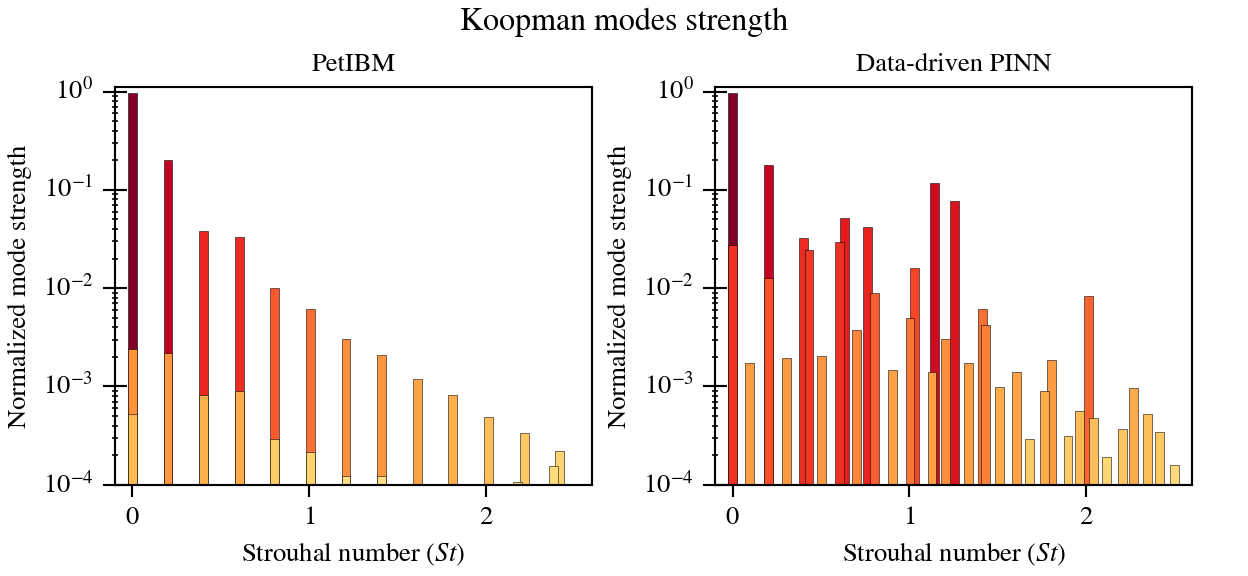
\includegraphics[width=0.975\linewidth]{cylinder-2d-re200/koopman/koopman_mode_strength}
    \caption{2D Cylinder, $Re=200$: Koopman mode strength v.s. Strouhal number}
    \label{fig:koopman-freq-st}
\end{figure}

Figure \ref{fig:koopman-freq-st} shows mode strengths versus mode frequencies.
The plots use nondimensional frequency, i.e., Strouhal number $St\equiv\frac{Df}{U_{inlet}}$, in their horizontal axes. 
In our cylinder flow, $D=U_{inlet} = 1$.
We only plotted modes with $f_j \ge 0$ for a concise visualization.
Note that we use a log scale for the vertical axis.
Plots in this figure also show the same observations in the previous paragraphs: the data-driven PINN is more dispersive and dissipative.

An observation that is now clearer from figure \ref{fig:koopman-freq-st} is the strength distribution.
In PetIBM's plot, strengths decrease exponentially from the steady mode (i.e., $St=0$) to high-frequency modes.
One can deduce a similar conclusion from PetIBM's simulation result.
The vortex shedding is dominated by a single frequency (this frequency is $St\approx 0.2$ because $t\in[125, 140]$ contains three periods).
Therefore, the flow should be dominated by the steady mode and a mode with a frequency close to $St=0.2$.
We can indeed verify this statement from PetIBM's plot in figure \ref{fig:koopman-freq-st}: the primary modes of $St=0$ and $St\approx 0.2$ are much stronger than others.
The strength of the immediately next mode, i.e., $St\approx 0.4$, drops in an order of magnitude. 
Note the use of the logarithm scale.
If we re-plot figure \ref{fig:koopman-freq-st} using a regular scale, only $St=0$ and $St=0.2$ would be visible in the figure.

The strength distribution in the PINN's plot also shows that $St=0$ and $St\approx 0.2$ are strong.
However, they are not the only dominating modes.  
Some other modes also have strengths at around $10^{-1}$.
As discovered in the previous paragraphs, these additional strong modes are damped modes.
We also observed that some damped modes have the same frequencies as primary modes.
For example, the secondary modes at $St=0$ and $St=0.2$ are damped modes, which can be confirmed in figure \ref{fig:koopman-eigval-dist}.
Note that for $St=0$, if a mode is damped, then it is not a steady mode anymore because its magnitude changes with time, though it is still non-oscillating.

\begin{table}[hbt!]
    \singlespacing
    \begin{threeparttable}[b]
        \begin{tabular}{ccccc}
            \toprule
            $St$ & Strength\tnote{1} & Growth Rate & Contours \\
            \midrule
            0     & 0.96 & 1.3e-7  & Figure \ref{fig:koopman-petibm-mode-1}\\
            0.201 & 0.20 & -4.3e-7 & Figure \ref{fig:koopman-petibm-mode-2}\\
            0.403 & 0.04 & 1.7e-6  & Figure \ref{fig:koopman-petibm-mode-3}\\
            0.604 & 0.03 & 2.7e-6  & Figure \ref{fig:koopman-petibm-mode-4}\\
            \bottomrule
        \end{tabular}%
        \begin{tablenotes}
            \footnotesize
            \item [1] Normalized.
        \end{tablenotes}
        \caption{%
            2D Cylinder, $Re=200$: top 4 primary dynamic modes (sorted by strengths) for PetIBM%
        }%
        \label{table:koopman-petibm}
    \end{threeparttable}
\end{table}%

Table \ref{table:koopman-petibm} summarizes the top 4 modes (ranked in their strengths) in PetIBM's spectral result.
For reference, these modes' contours are provided in figure \ref{fig:koopman-petibm-mode-1} to \ref{fig:koopman-petibm-mode-4}.
The dynamic modes are complex-valued, and the contours include both the real and the imaginary parts.
Note the growth rates of these 4 modes are not exactly zero but around $10^{-6}$ and $10^{-7}$.
We were unsure if we could treat them as zero at these orders of magnitude.
If not, and if they do cause the primary modes to be slightly damped or augmented over time, then we believe they also serve a reasonable explanation for the existence of the other 50 non-primary modes in PetIBM---to compensate for the loss or the gain in the primary modes.

Table \ref{table:koopman-pinn-non-damped} lists the PINN's top 4 primary modes. They are the same as those in table \ref{table:koopman-petibm}.
Table \ref{table:koopman-pinn-damped} shows the top 4 damped modes in the PINN's result.
Their contours are also indicated in the tables for readers' reference.
The growth rates of the primary modes in the PINN's result are around $10^{-5}$ and $10^{-6}$, slightly larger than that of PetIBM's.
If these orders of magnitude can not be deemed as zero, then these primary are slightly damped and dissipative, though the major source of the numerical dissipation may still be the actual damped modes in table \ref{table:koopman-pinn-damped}.

\begin{table}[hbt!]
    \singlespacing
    \begin{threeparttable}[b]
        \begin{tabular}{ccccc}
            \toprule
            $St$ & Strength\tnote{1} & Growth Rate & Contours \\
            \midrule
            0     & 0.97 & -2.2e-6  & Figure \ref{fig:koopman-pinn-undamped-mode-1}\\
            0.201 & 0.18 & -9.4e-6 & Figure \ref{fig:koopman-pinn-undamped-mode-2}\\
            0.403 & 0.03 & 2.3e-5  & Figure \ref{fig:koopman-pinn-undamped-mode-3}\\
            0.604 & 0.03 & -8.6e-5  & Figure \ref{fig:koopman-pinn-undamped-mode-4}\\
            \bottomrule
        \end{tabular}%
        \begin{tablenotes}
            \footnotesize
            \item [1] Normalized.
        \end{tablenotes}
        \caption{%
            2D Cylinder, $Re=200$: top 4 primary dynamic modes (sorted by strengths) for PINN%
        }%
        \label{table:koopman-pinn-non-damped}
    \end{threeparttable}
\end{table}%

\begin{table}[hbt!]
    \singlespacing
    \begin{threeparttable}[b]
        \begin{tabular}{ccccc}
            \toprule
            $St$ & Strength\tnote{1} & Growth Rate & Contours \\
            \midrule
            1.142 & 0.12 & -0.24 & Figure \ref{fig:koopman-pinn-damped-mode-1}\\
            1.253 & 0.08 & -0.22 & Figure \ref{fig:koopman-pinn-damped-mode-2}\\
            0.633 & 0.05 & -0.14 & Figure \ref{fig:koopman-pinn-damped-mode-3}\\
            0.761 & 0.04 & -0.13 & Figure \ref{fig:koopman-pinn-damped-mode-4}\\
            \bottomrule
        \end{tabular}%
        \begin{tablenotes}
            \footnotesize
            \item [1] Normalized.
        \end{tablenotes}
        \caption{%
            2D Cylinder, $Re=200$: top 4 damped dynamic modes (sorted by strengths) for PINN%
        }%
        \label{table:koopman-pinn-damped}
    \end{threeparttable}
\end{table}%

\begin{figure}[hbt!]
    \centering
    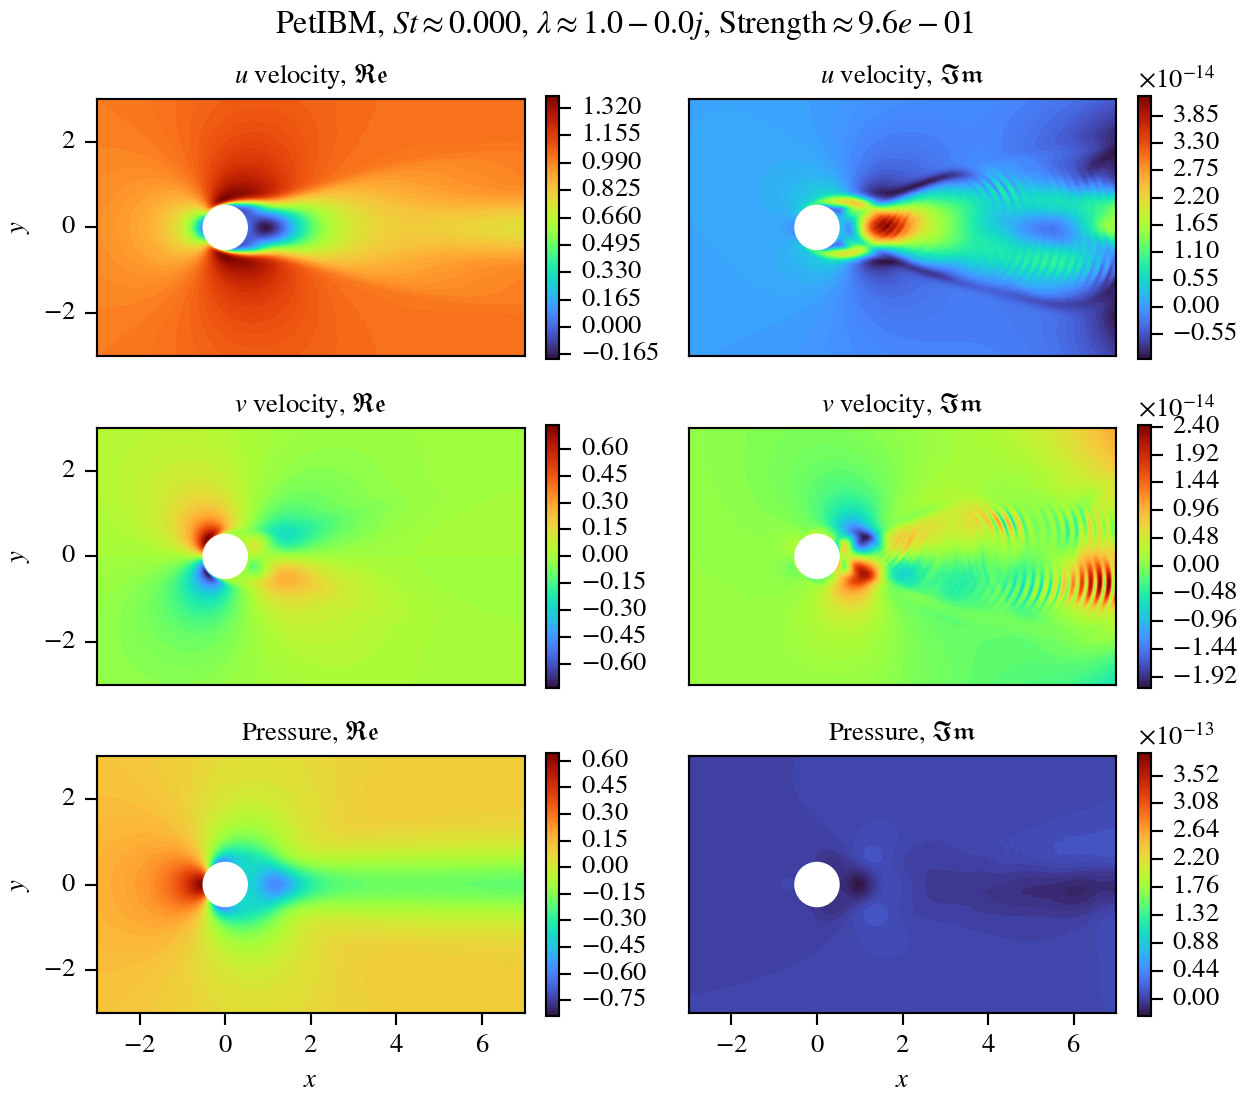
\includegraphics[width=0.975\linewidth]{cylinder-2d-re200/koopman/koopman_petibm_000_st0.000}
    \caption{2D Cylinder, $Re=200$: Koopman mode, $St=0$ (PetIBM)}
    \label{fig:koopman-petibm-mode-1}
\end{figure}

\begin{figure}[hbt!]
    \centering
    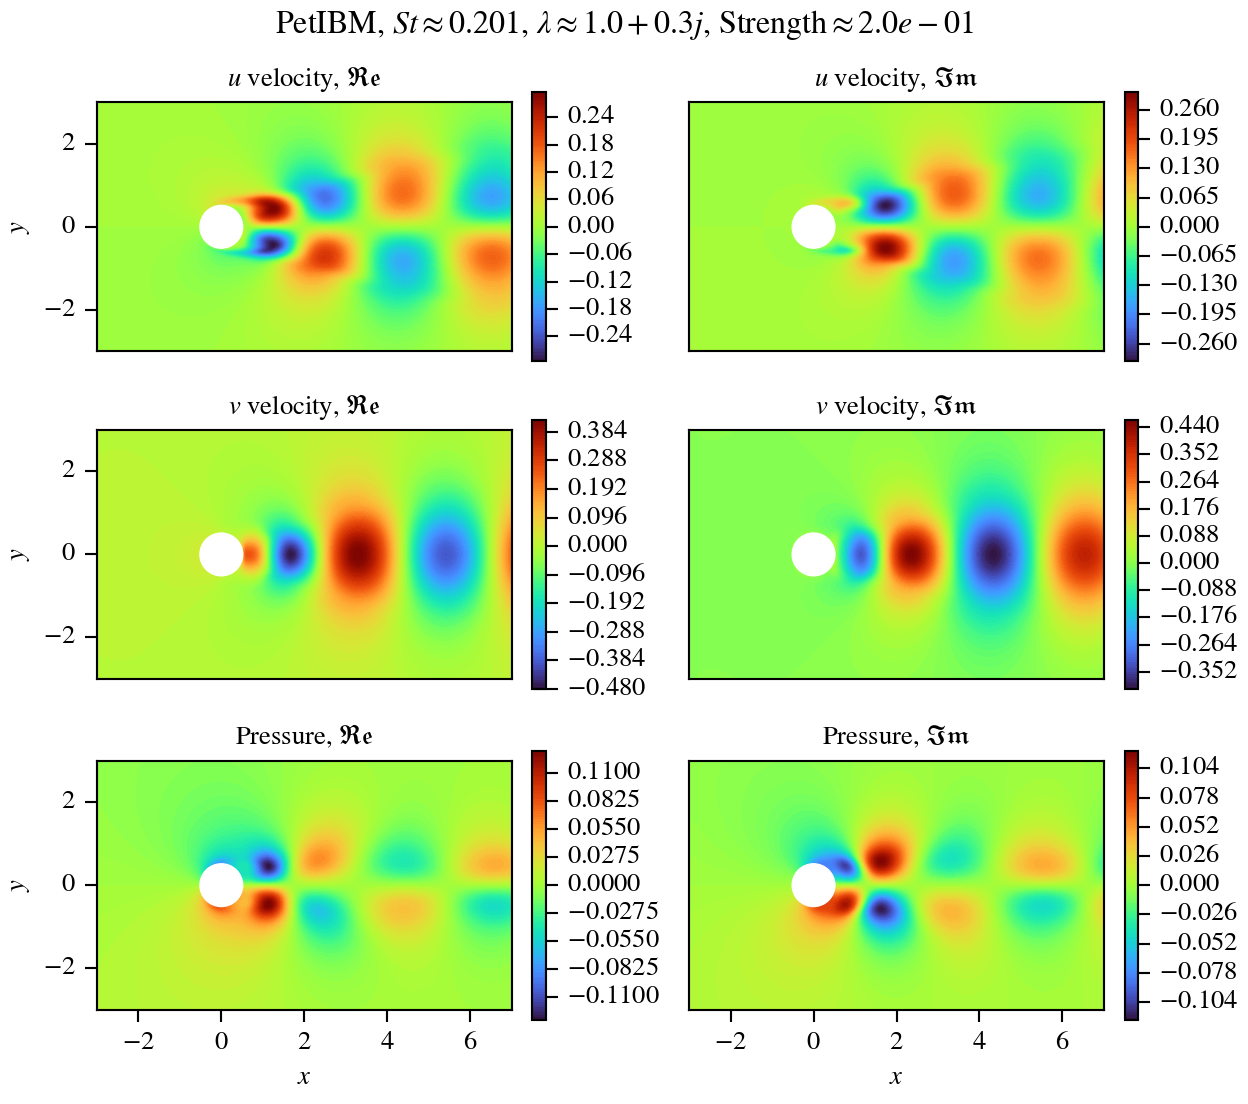
\includegraphics[width=0.975\linewidth]{cylinder-2d-re200/koopman/koopman_petibm_001_st0.201}
    \caption{2D Cylinder, $Re=200$: Koopman mode, $St=0.201$ (PetIBM)}
    \label{fig:koopman-petibm-mode-2}
\end{figure}

\begin{figure}[hbt!]
    \centering
    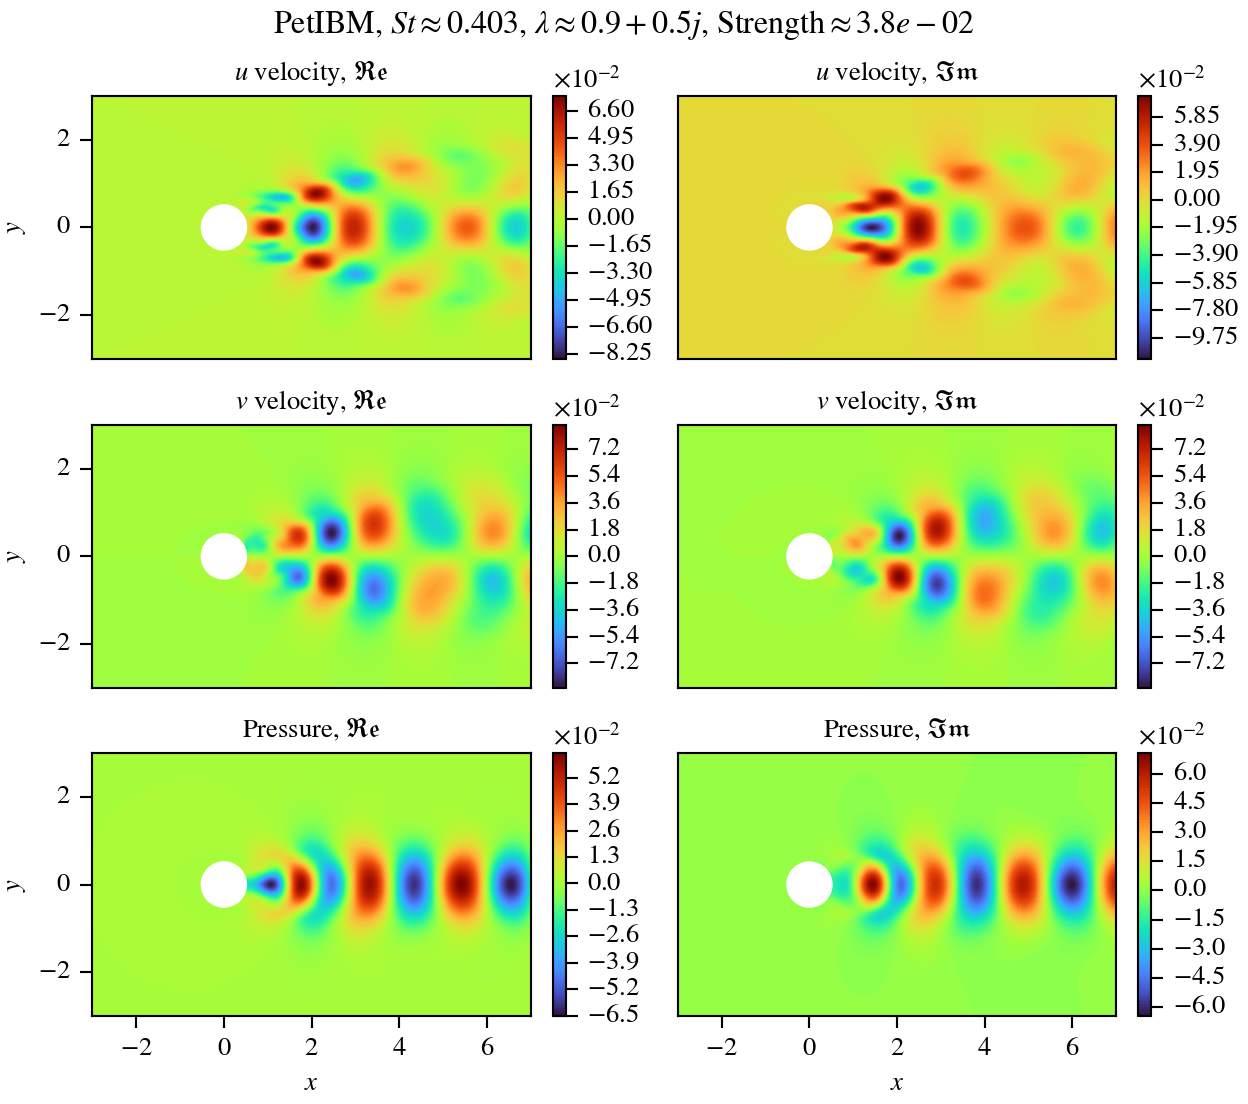
\includegraphics[width=0.975\linewidth]{cylinder-2d-re200/koopman/koopman_petibm_002_st0.403}
    \caption{2D Cylinder, $Re=200$: Koopman mode, $St=0.403$ (PetIBM)}
    \label{fig:koopman-petibm-mode-3}
\end{figure}

\begin{figure}[hbt!]
    \centering
    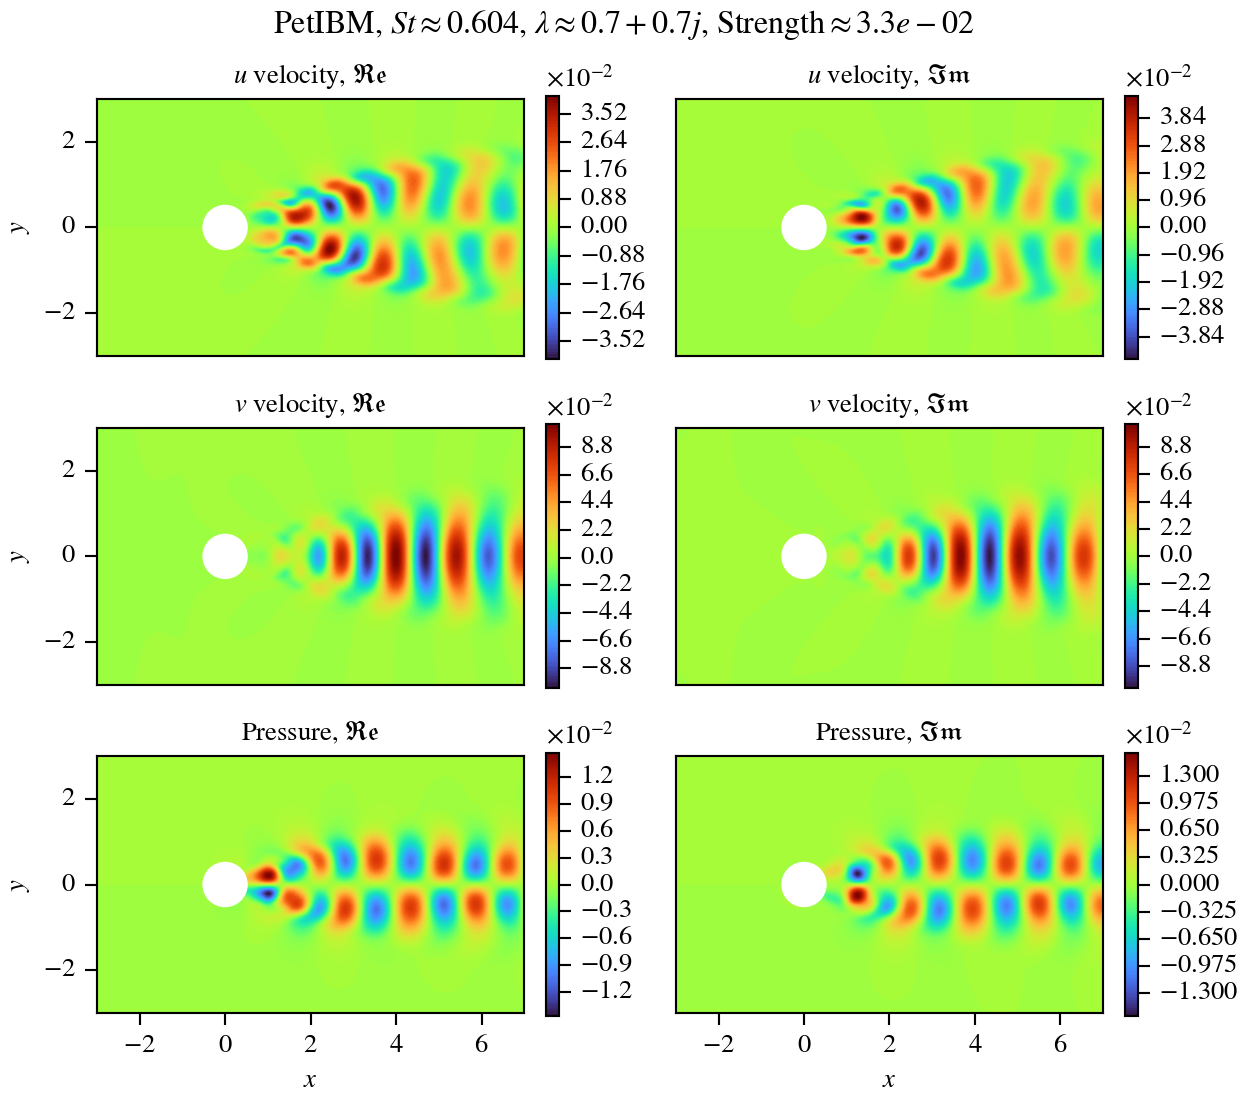
\includegraphics[width=0.975\linewidth]{cylinder-2d-re200/koopman/koopman_petibm_003_st0.604}
    \caption{2D Cylinder, $Re=200$: Koopman mode, $St=0.604$ (PetIBM)}
    \label{fig:koopman-petibm-mode-4}
\end{figure}

\begin{figure}[hbt!]
    \centering
    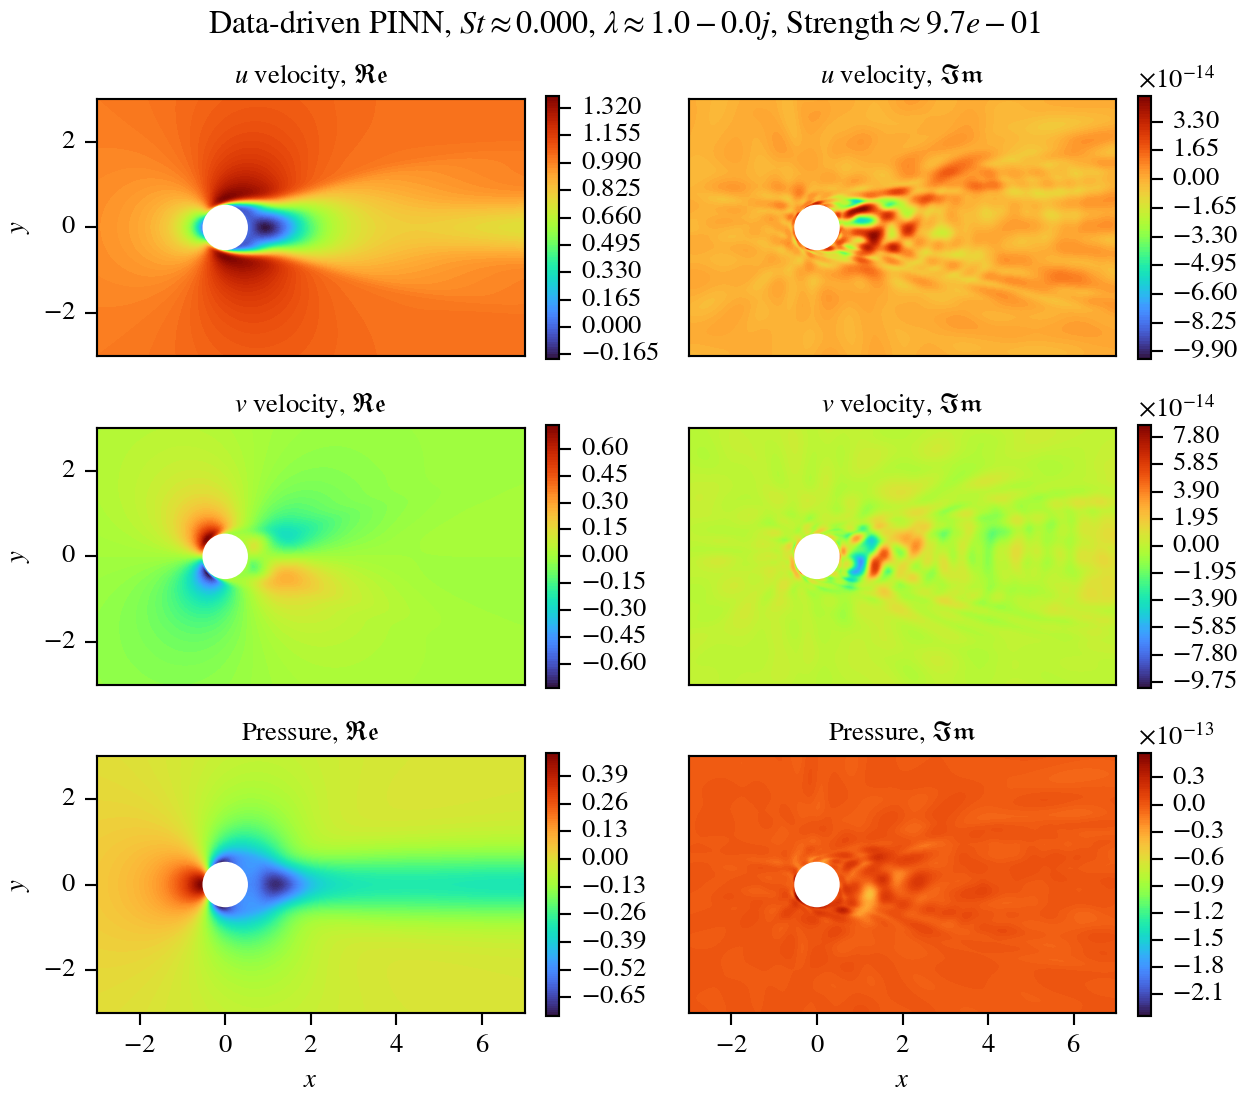
\includegraphics[width=0.975\linewidth]{cylinder-2d-re200/koopman/koopman_pinn_000_st0.000}
    \caption{2D Cylinder, $Re=200$: Koopman mode, $St=0$ (PINN)}
    \label{fig:koopman-pinn-undamped-mode-1}
\end{figure}

\begin{figure}[hbt!]
    \centering
    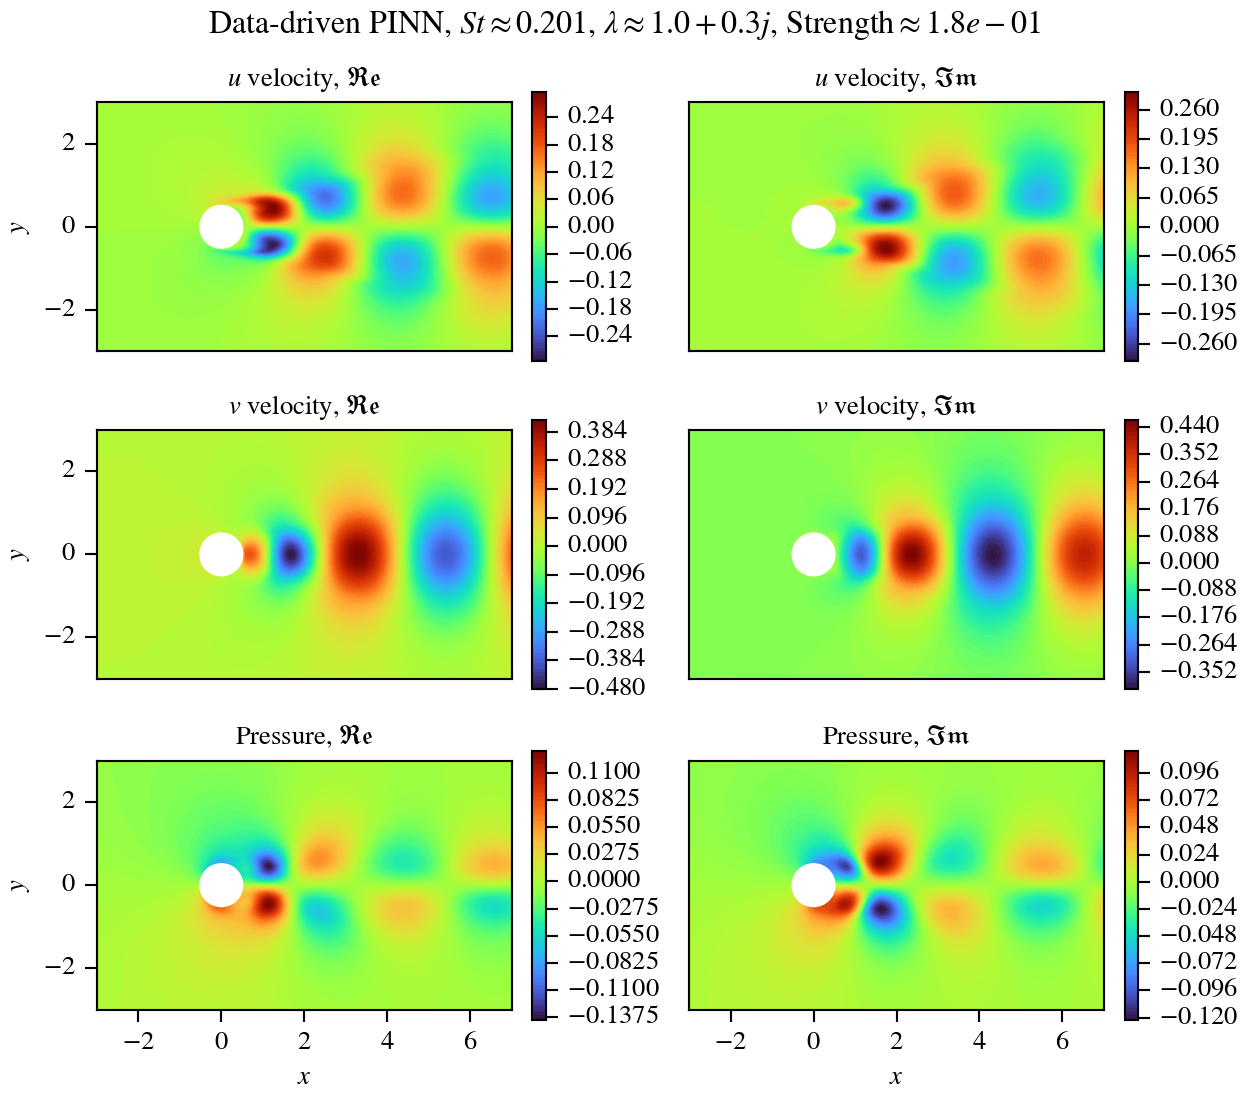
\includegraphics[width=0.975\linewidth]{cylinder-2d-re200/koopman/koopman_pinn_001_st0.201}
    \caption{2D Cylinder, $Re=200$: Koopman mode, $St=0.201$ (PINN)}
    \label{fig:koopman-pinn-undamped-mode-2}
\end{figure}

\begin{figure}[hbt!]
    \centering
    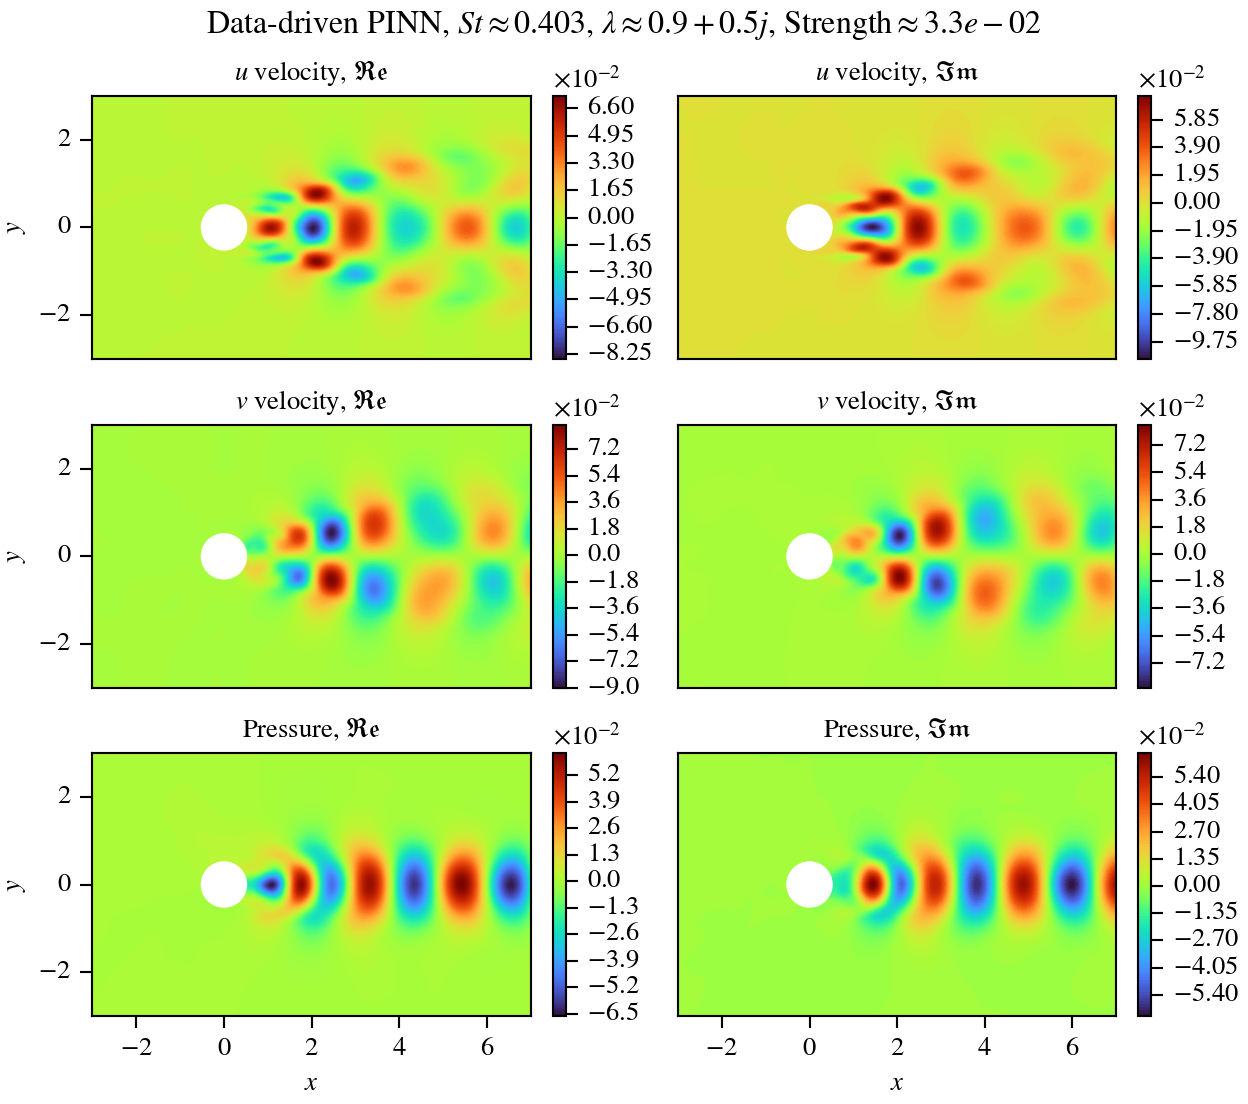
\includegraphics[width=0.975\linewidth]{cylinder-2d-re200/koopman/koopman_pinn_006_st0.403}
    \caption{2D Cylinder, $Re=200$: Koopman mode, $St=0.403$ (PINN)}
    \label{fig:koopman-pinn-undamped-mode-3}
\end{figure}

\begin{figure}[hbt!]
    \centering
    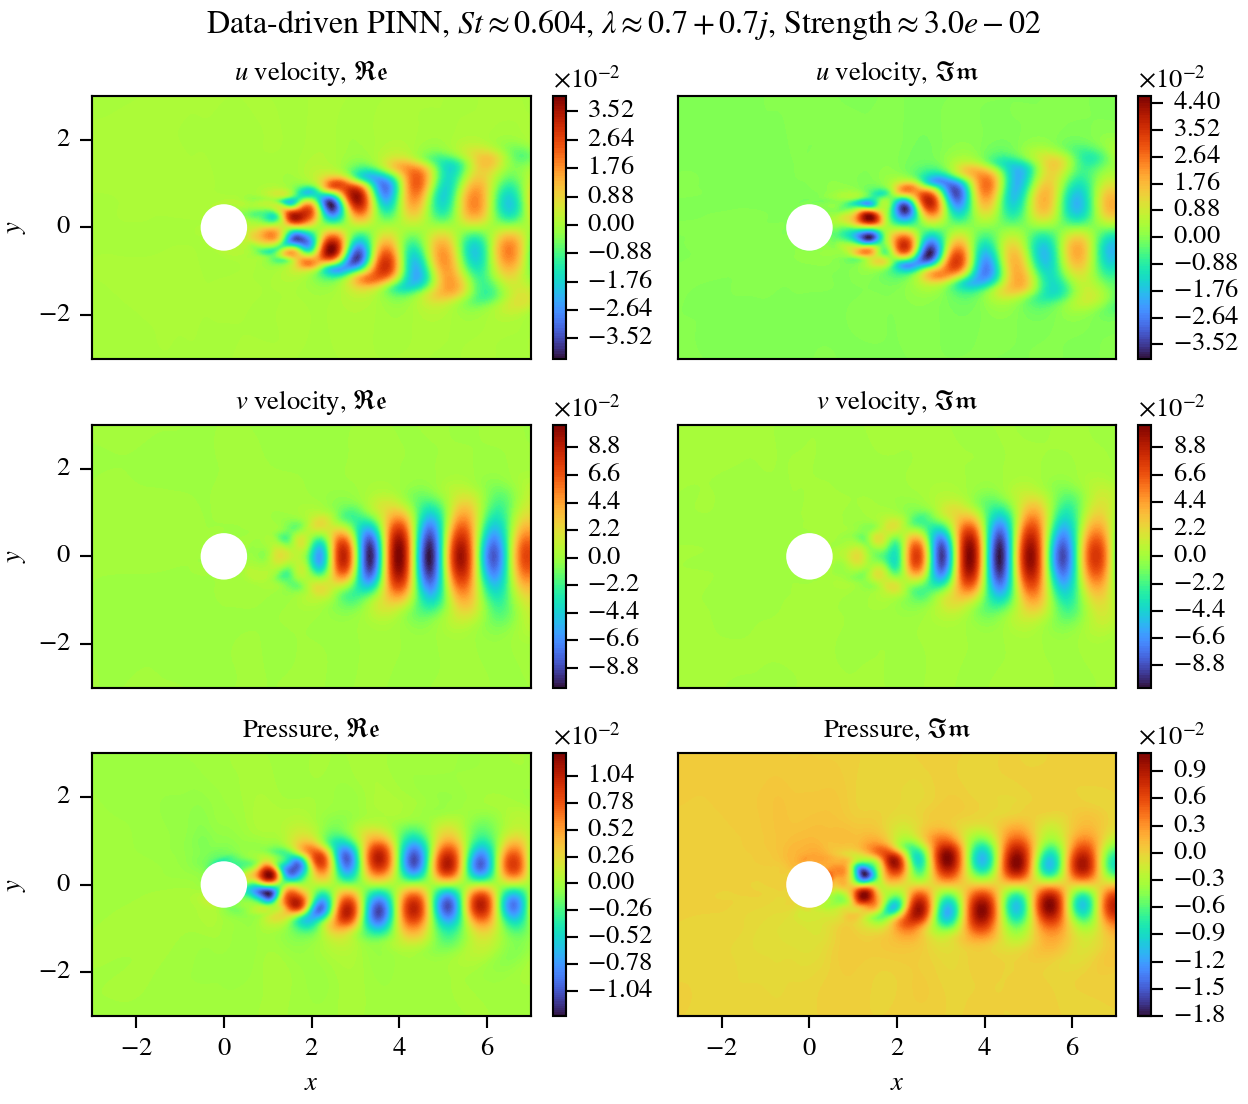
\includegraphics[width=0.975\linewidth]{cylinder-2d-re200/koopman/koopman_pinn_007_st0.604}
    \caption{2D Cylinder, $Re=200$: Koopman mode, $St=0.604$ (PINN)}
    \label{fig:koopman-pinn-undamped-mode-4}
\end{figure}

\begin{figure}[hbt!]
    \centering
    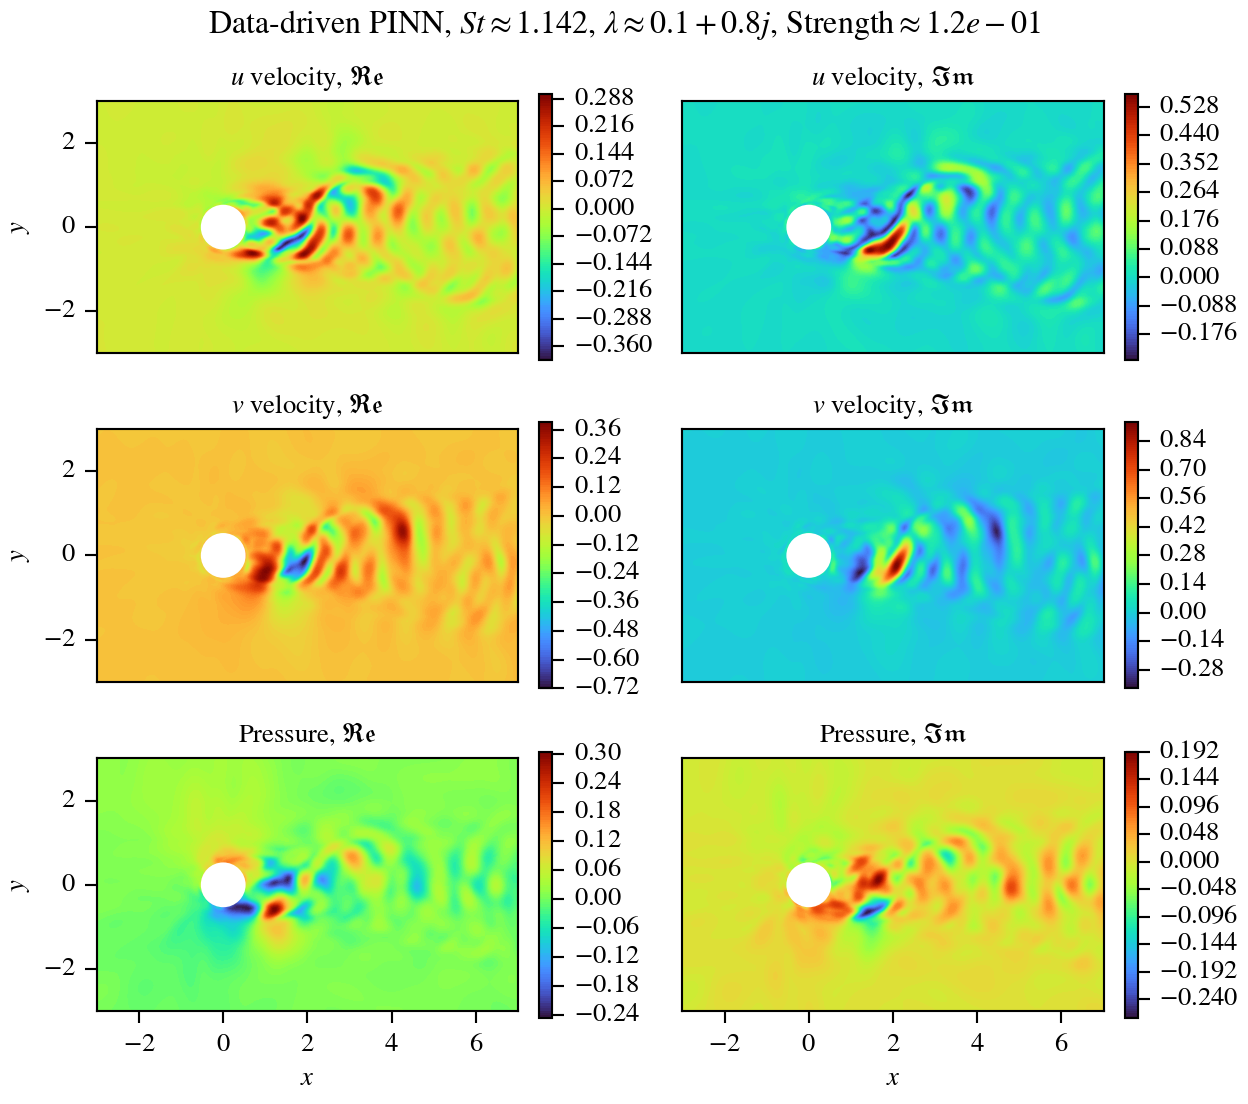
\includegraphics[width=0.975\linewidth]{cylinder-2d-re200/koopman/koopman_pinn_002_st1.142}
    \caption{2D Cylinder, $Re=200$: Koopman mode, $St=1.142$ (PINN)}
    \label{fig:koopman-pinn-damped-mode-1}
\end{figure}

\begin{figure}[hbt!]
    \centering
    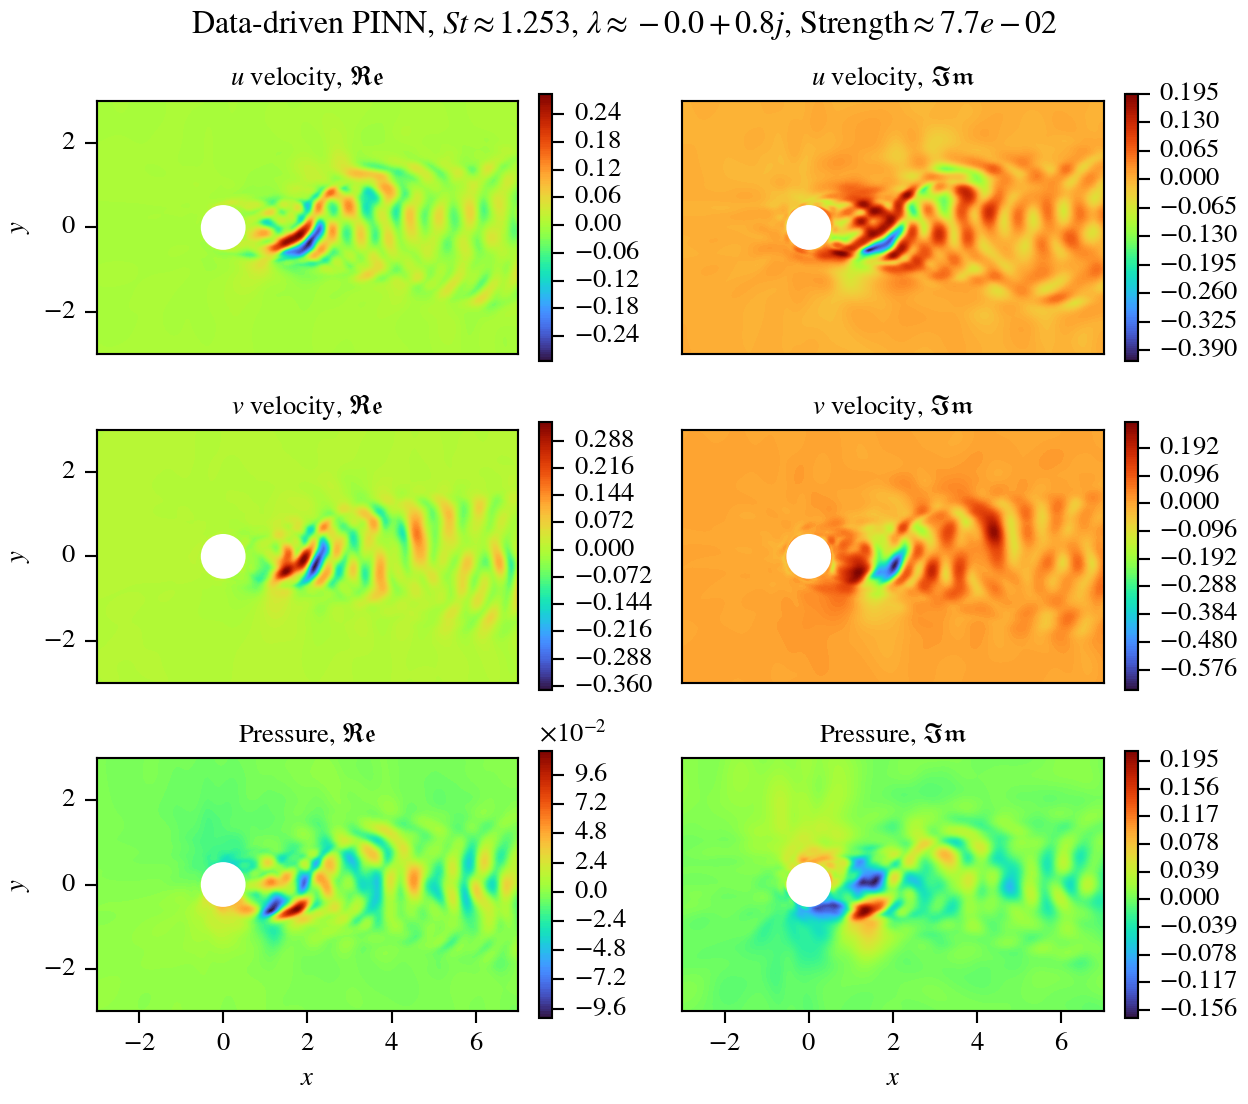
\includegraphics[width=0.975\linewidth]{cylinder-2d-re200/koopman/koopman_pinn_003_st1.253}
    \caption{2D Cylinder, $Re=200$: Koopman mode, $St=1.253$ (PINN)}
    \label{fig:koopman-pinn-damped-mode-2}
\end{figure}

\begin{figure}[hbt!]
    \centering
    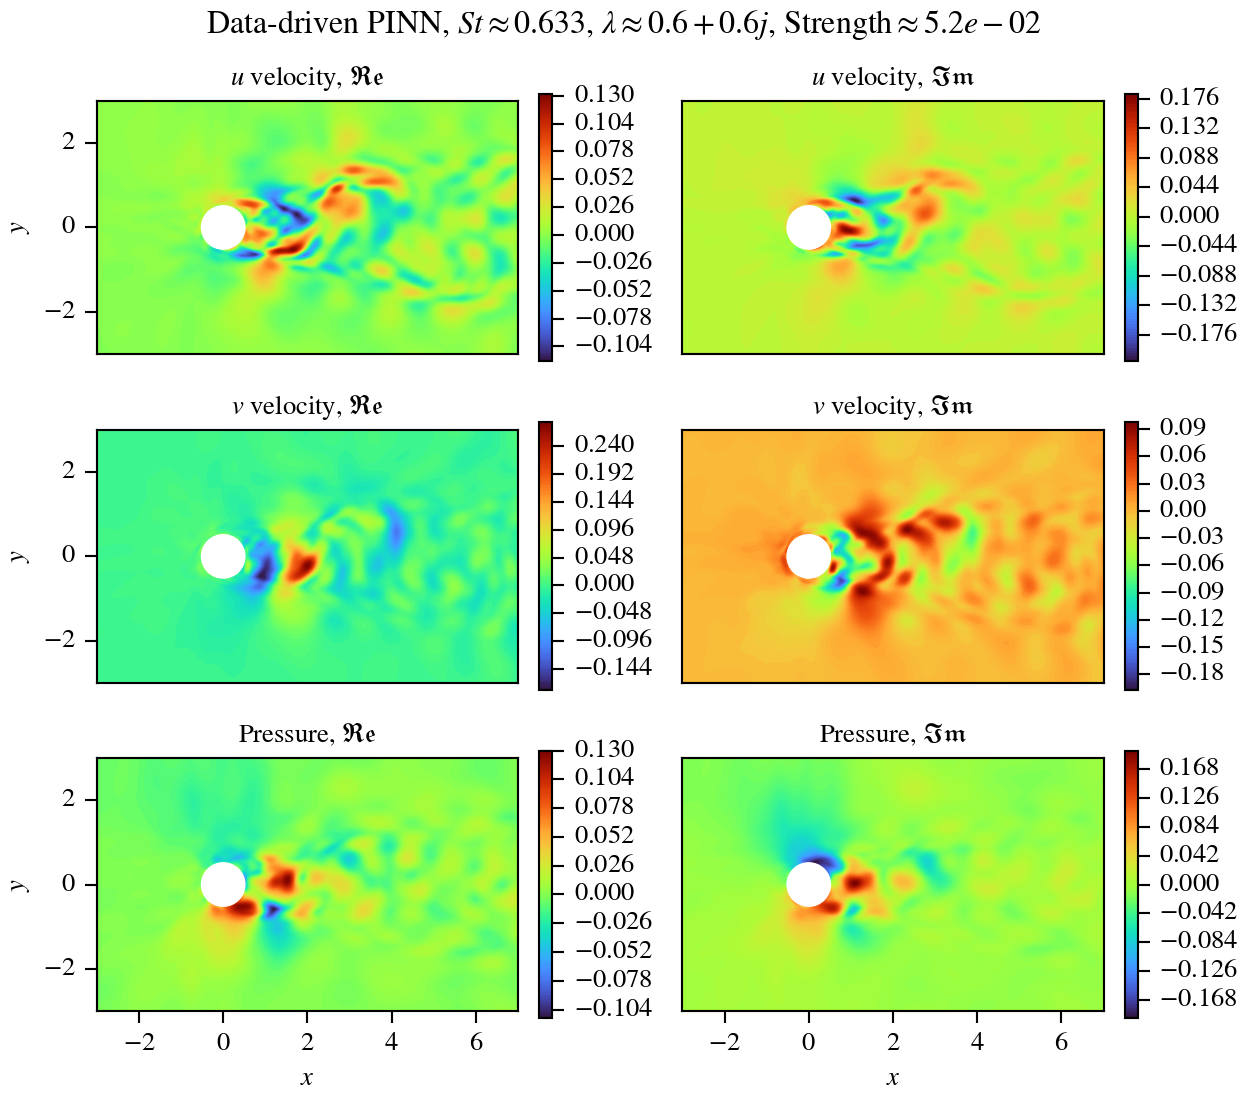
\includegraphics[width=0.975\linewidth]{cylinder-2d-re200/koopman/koopman_pinn_004_st0.633}
    \caption{2D Cylinder, $Re=200$: Koopman mode, $St=0.633$ (PINN)}
    \label{fig:koopman-pinn-damped-mode-3}
\end{figure}

\begin{figure}[hbt!]
    \centering
    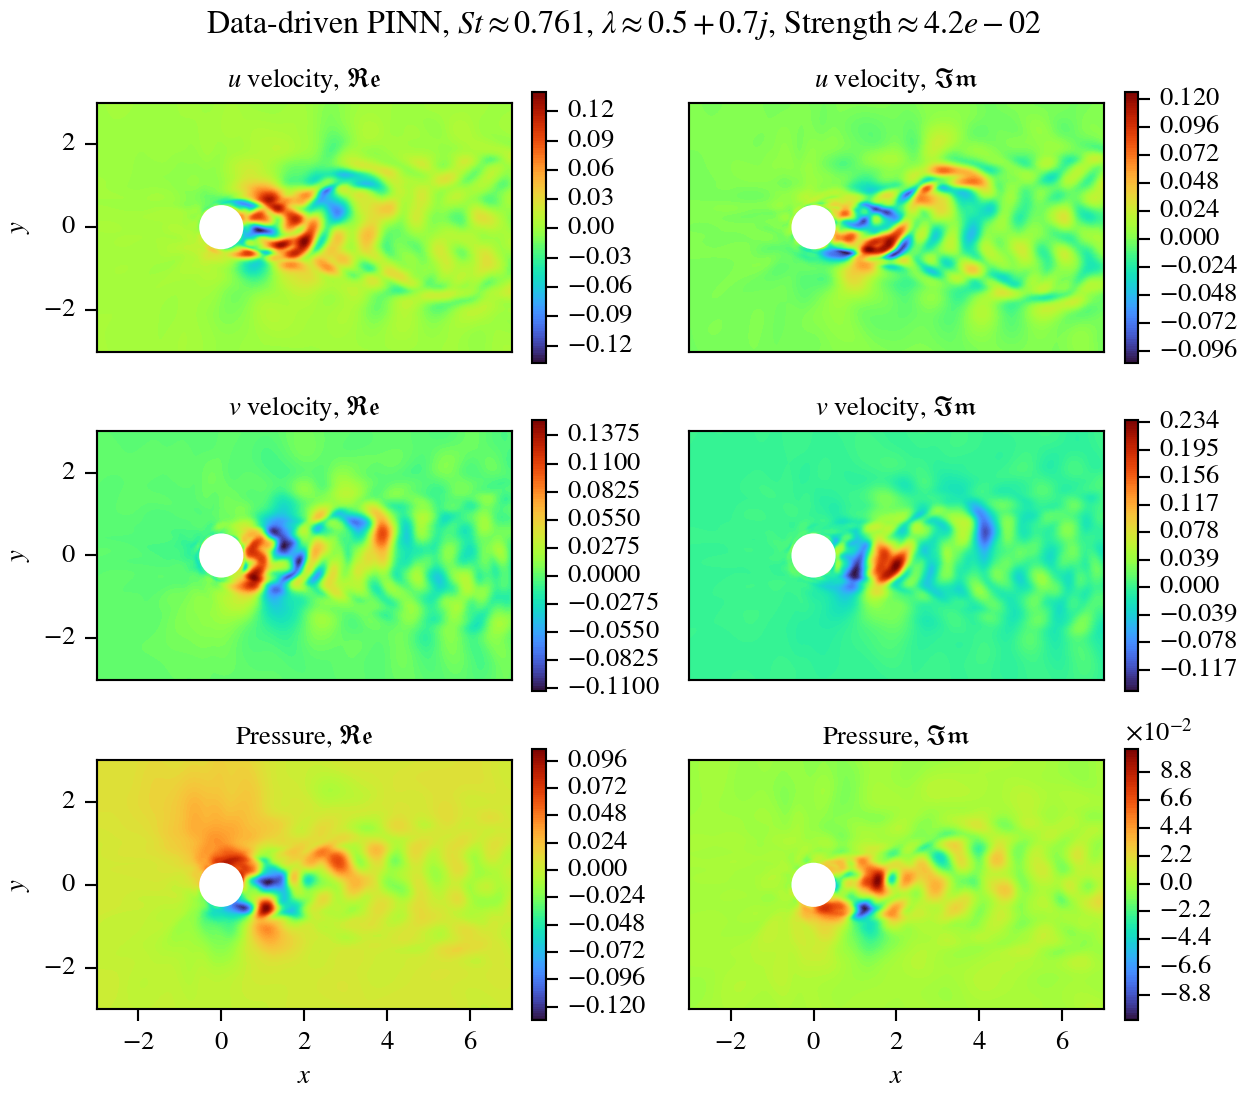
\includegraphics[width=0.975\linewidth]{cylinder-2d-re200/koopman/koopman_pinn_005_st0.761}
    \caption{2D Cylinder, $Re=200$: Koopman mode, $St=0.761$ (PINN)}
    \label{fig:koopman-pinn-damped-mode-4}
\end{figure}

% vim:ft=tex
